\documentclass[11pt]{article}

\usepackage[utf8]{inputenc}
\usepackage[margin=1in]{geometry}
\usepackage{amsmath,amssymb}
\usepackage{multicol}
\usepackage{enumerate}
\usepackage{graphicx}
\usepackage{spalign}
\usepackage{hyperref}
\setlength{\parindent}{0pt}
\usepackage{listings} 
\usepackage{mdframed}
\usepackage{systeme}
\usepackage{amsmath}
\usepackage[colorinlistoftodos]{todonotes}
\usepackage{amssymb}
\usepackage{marginnote}
\usepackage{float}
\usepackage{subfig}
\usepackage{enumerate}
\usepackage{amsfonts}
\usepackage{amssymb}
\usepackage{mathrsfs}
\usepackage{dsfont}
\usepackage{algorithm}
\usepackage{algpseudocode}
\usepackage{pifont}


%%	 MATLAB
\usepackage[framed,numbered,autolinebreaks,useliterate]{mcode}

% Document layout
\geometry{a4paper, margin=1in}

\title{Predicting the Financial Success of Will Ferrell Movies}
\author{Nicholas Mankowski}
\date{December 13, 2023} % You can set a specific date like \date{December 1, 2023}


\renewcommand{\theenumi}{\Alph{enumi}}
\newcommand{\phanmin}{\phantom{-}}
\renewcommand{\vec}[1]{\mathbf{#1}}

\begin{document}

\maketitle

In the competitive and unpredictable world of film, Will Ferrell has managed to build a vast portfolio of movies across many genres, creating multiple box-office hits in the process. But what really makes a Will Ferrell movie successful? In this paper, we will be predicting the success of a Will Ferrell movie measured in final box office sales.  
We will use IMDb ratings, Rotten Tomatoes Scores, Will Ferrell's age, as well as the production cost of the movie to predict this success. 
Parsing data from the Rotten Tomatoes site dedicated to Will Ferrell, we will randomly select 10 distinct movies to pull data from. 
Using the corresponding data from these 10 movies, we will build 5 models to predict the total box office sales of future movies casting Will Ferrell.  
Comparing the outcomes predicted by these models to actual data, we will also analyze their effective at predicting financial success of movies casting Will Ferrell.

\section{\centering Will Ferrell Movie Data}
\label{movie-data}


\subsection{\centering Means of Data Collection} % TODO: Citations?
The movies were picked from a list of Will Ferrell's movies in order of their Rotten Tomatoes score.  
A Python script was developed to extract movie data—including Movie Title, Year, and Rotten Tomatoes Score—from the HTML of the corresponding website.
From this list of movies, the script picks 10 distinct and random movies that were released in or after 2000.  
From here, the production cost of the movie, IMDb rating, as well as final box office sales were found from the IMDb website.  
If no data was found, the movie was substituted for another randomly pulled movie pulled from the list that does have the aforementioned data included.
The dollar amounts listed were then adjusted for inflation and listed in millions and the age of Will Ferrell at the time of release was calculated.
\subsection{\centering Raw Will Ferrell Movie Data}
    %TODO: Fix centering here
    \begin{table}[H]
        \centering
        \scriptsize
        \caption{Rotten Tomatoes Score, IMDb Rating, and Age of Will Ferrell at Time of Movie Release.}
        \begin{tabular}{|l|r|r|r|}
        %\cline{1-4}
        \hline
        \textbf{Title}                         & \multicolumn{1}{l|}{\textbf{Rotten Tomatoes Score}} & \multicolumn{1}{l|}{\textbf{IMDb Rating}} & \multicolumn{1}{l|}{\textbf{Will Ferrell Age}} \\ \hline%\cline{1-4}
        Daddy's Home 2                        & 21\%                                       & 6                                & 50                                    \\ \hline%\cline{1-4}
        Holmes \& Watson                      & 10\%                                       & 3.9                              & 51                                    \\ \hline%\cline{1-4}
        Bewitched                             & 24\%                                       & 4.8                              & 38                                    \\ \hline%\cline{1-4}
        The LEGO Movie 2: The Second Part     & 84\%                                       & 6.6                              & 52                                    \\ \hline%\cline{1-4}
        The Other Guys                        & 79\%                                       & 6.6                              & 43                                    \\ \hline%\cline{1-4}
        Anchorman: The Legend of Ron Burgundy & 66\%                                       & 7.1                              & 37                                    \\ \hline%\cline{1-4}
        Zoolander                             & 65\%                                       & 6.5                              & 34                                    \\ \hline%\cline{1-4}
        Kicking \& Screaming                  & 41\%                                       & 5.6                              & 38                                    \\ \hline%\cline{1-4}
        Semi-Pro                              & 23\%                                       & 5.8                              & 41                                    \\ \hline%\cline{1-4}
        Get Hard                              & 28\%                                       & 6                                & 48                                    \\ \hline%\cline{1-4}
        \end{tabular}
    \end{table}

    \begin{table}[H]
        \centering
        \scriptsize
        \caption{Production Cost and Final Box Office Sales in Millions and Adjusted for Inflation}
        \begin{tabular}{|l|r|r|}
        \hline
        \textbf{Title}                                 & \multicolumn{1}{l|}{\textbf{Production Cost(nillions)}} & \multicolumn{1}{l|}{\textbf{Final Box Office Sales(millions)}} \\ \hline
        Daddy's Home 2                        & \$86.05                                                                & \$225.24 \\ \hline
        Holmes \& Watson                      & \$51.13                                                                & \$49.26  \\ \hline
        Bewitched                             & \$133.05                                                               & \$205.71 \\ \hline
        The LEGO Movie 2: The Second Part     & \$118.38                                                               & \$238.67 \\ \hline
        The Other Guys                        & \$140.19                                                               & \$238.97 \\ \hline
        Anchorman: The Legend of Ron Burgundy & \$42.07                                                                & \$146.79 \\ \hline
        Zoolander                             & \$45.31                                                                & \$98.36  \\ \hline
        Kicking \& Screaming                  & \$70.44                                                                & \$87.76  \\ \hline
        Semi-Pro                              & \$78.09                                                                & \$62.48  \\ \hline
        Get Hard                              & \$51.59                                                                & \$144.08 \\ \hline
        \end{tabular}
    \end{table}

\section{\centering Modeling Movie Data}
\subsection{One Variable Linear Model}
\subsubsection{Description of Mathematics}
\label{one-variable-math-desc}
For our one variable linear model, we are building a linear regression model of the form
\begin{equation*}
    F = a_1 + a_2 B \, ,
\end{equation*}
where $F$ is the final box office sales of a movie, $B$ is the production cost of said movie, and $a_1, a_2$ are coefficients that minimize the error of our regression line.
We can describe the error of our model at each point by looking at the difference in expected result vs. actual result, which yields
\begin{equation*}
    E_i = F_i - a_1 - a_2 B_i \, ,
\end{equation*}
where $F_i$ is the final box office sale of an individual movie, $B_i$ is the budget of said movie, and $E_i$ is the error in our prediction. 
\\

Furthermore, we can sum the squared difference of each of the $n$ movie results to produce the ordinary least squares method of error calculation, which we can write as a function of our coefficients $a_1$ \& $a_2$:

\label{one-var-linear-ols-error}
\begin{equation*}
    E(a_1, a_2) = \sum_{i=1}^{n}(F_i - a_1 - a_2 B_i)^2 \, .
\end{equation*}

Notice that if we want to find the coefficients that minimize our value of $E$, we can find the partial derivatives of $E$ with respect to $a_1$ as well as $a_2$ and find where these derivatives are equal to zero.  
This will give us a system of equations that we could use to solve for the $a_1, a_2$ that minimize $E$.  
Applying this, we get

% TODO: show that we are actually finding a minimum

\begin{align*}
    \frac{\partial E(a_1, a_2)}{\partial a_1} = 0 & \implies \sum_{i=1}^{n} -2 (F_i - a_1 - a_2 B_i) = 0\, ,\\
    \frac{\partial E(a_1, a_2)}{\partial a_2} = 0 & \implies \sum_{i=1}^{n} -2 B_i (F_i - a_1 - a_2 B_i) = 0\,.
\end{align*}

We can rewrite this system of equations as the following:

\begin{align*}
    \sum_{i=1}^{n}F_i & = n a_1 + a_2 \sum_{i=1}^{n}B_i \\ % TODO: maybe spend more time formatting it to look more like a system of equations
    \sum_{i=1}^{n}B_i F_i & = a_1 \sum_{i=1}^{n} B_i + a_2 \sum_{i=1}^{n} B_i^2 \, .
\end{align*}
Expressed as a matrix, we have the system of equations to be
\label{one-variable-error-matrix-1}
\begin{equation*}
    \begin{bmatrix}
        \sum_{i=1}^{n}F_i \\
        \sum_{i=1}^{n}B_i F_i
    \end{bmatrix}
    =
    \begin{bmatrix}
        n & \sum_{i=1}^{n} B_i \\
        \sum_{i=1}^{n} B_i & \sum_{i=1}^{n} B_i^2
    \end{bmatrix} 
    \begin{bmatrix}
        a_1 \\
        a_2
    \end{bmatrix} \, .
\end{equation*}

Thus, we can solve for $a_1$ and $a_2$ in the above to get the coefficients that minimize the least squares error in our linear regression model. % TODO: say why we can solve for a_1 & a_2??  do we have to say that the 2x2 is invertible?

\subsubsection{Application in Code}
We can follow the above steps to find the values of $a_1, a_2$ to minimize our least squares error using the \texttt{polyfit} function in MATLAB.
\label{polyfit-degree-1}
\begin{lstlisting}
% Get our coeficients a_1, a_2
coef = polyfit(cost, sales, 1); 
\end{lstlisting}
Looking at the results of \texttt{polyfit} specifying degree \texttt{1}, we get the values
\[ a_1 = 30.750329, a_2 = 1.457573 \, .\]
Note: \texttt{polyfit} returns the values in order of the highest order to lowest order, so the vector \texttt{coef} will look like \texttt{[a\_2, a\_1]}. 
\\

Hence, we can see that we now have this explicit equation for our model:
\[ F = 30.750329 + 1.457573 B \, .\]
Now, we can evaluate our model by using the \texttt{polyval} function at cost $b$ as follows:
\label{assemble-model-polyval}
\begin{lstlisting}
% Assemble our model for a given cost b
model = @(b) polyval(coef, b);
\end{lstlisting}
To build a visualization of our model, we can simulate a continuous expression of time using a small step size, and then evaluate the model at each time step.
\label{create-visualization}
\begin{lstlisting}
% Create a domain for the models
timeCts = 0:0.1:150;
% Create the models
cost_visualization = model(timeCts);
\end{lstlisting}
Furthermore, we can plot our model using the following MATLAB code:
\label{model-plotting}
\begin{lstlisting}
hold on;
% Plot the raw data
scatter(cost, sales, 'DisplayName', 'Raw Data');
% Plot our model
plot(timeCts, cost_visualization, 'DisplayName', 'Linear Regression Model');
% Set limits to properly showcase our graph
xlim([0, 150]);
ylim([0, 300]);
% Label and title the graph accordingly
xlabel('Production Cost of Movie Adjusted for Inflation(millions)');
ylabel('Final Box Office Sales of Movie Adjusted for Inflation(millions)');
title('Cost vs. Final Box Office Sales of a Will Ferrell Movie');
% Show the legend
legend;
hold off;
\end{lstlisting}

\subsubsection{Model Analysis}
\label{one-variable-linear-model-analysis}
As a result of the model visualization presented in \ref{model-plotting}, we obtain the following result:
\begin{figure}[H]
    \centering 
    \label{one-variable-linear-plot}
    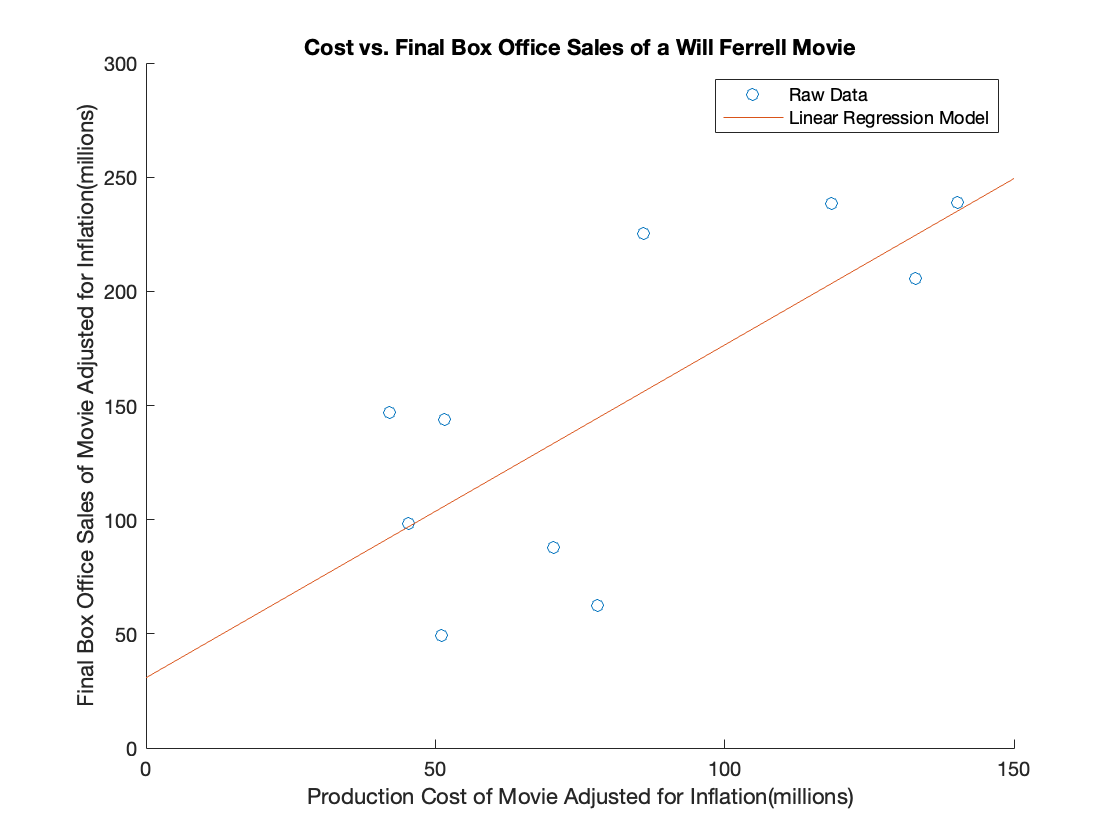
\includegraphics[width=\textwidth]{models/a.png}
\end{figure}
As seen above, the model seems to accurately describe the relationship between production cost and final box office sales.  
If we were to evaluate the error as described in \ref{one-var-linear-ols-error}, we can see that $E(30.750329, 1.457573) = 22808.960460$. 
Despite the error seeming rather high when quantified and also perhaps visually, when we look at the scale of values involved in this situation, it actually appears to be rather good.  
The model seems to fit our data well and trend in the correct direction.  
Looking further at the model, we can see that it makes intuitive sense.  
Our model suggests a positive correlation between production cost and final box office sales of a Will Ferrell movie.  
If the producers of a Will Ferrell movie invest more in quality production, they are likely to see higher box office returns. 
\\

% TODO: why doesn't \indent work?
Another interesting question is whether or not the relationship between production cost and box office sales is linear.  
When we think of investing in the terms of every day life, there is often an expectation of returns being compounded.  
This, of course, is often spread over time, so it makes intuitive and mathematical sense that our returns are non linear. 
This idea of investing may effect our intuition and incline us to believe the more accurate model for these data points is nonlinear, but is that really the case?
This question will be explored further at a later point in this paper.

\subsection{One Variable Quadratic Model}
\subsubsection{Description of Mathematics}
Similarly, we can extend the ideas discussed in \ref{one-variable-math-desc} to a one variable quadratic model of the form
\begin{align*}
    F = a_1 + a_2 B + a_2 B^2 \, .
\end{align*}
We can see that the least squares error of this will now be the following function of $a_1, a_2, a_3$:
\begin{align*}
    E(a_1, a_2, a_3) = \sum_{i=1}^{n}(F_i - a_1 - a_2 B_i - a_3 B_i^2)^2 \, .
\end{align*}
Hence, we can apply the ideas explored in \ref{one-var-linear-ols-error} to find the $a_1, a_2, \; \& \; a_3$ that minimize E.  Deriving with respect to $a_1, a_2, a_3$ and setting each to zero, we get 
\begin{align*}
    \frac{\partial E(a_1, a_2, a_3)}{\partial a_1} = 0 & \implies \sum_{i=1}^{n} -2 (F_i - a_1 - a_2 B_i - a_3 B_i^2) = 0, \\
    \frac{\partial E(a_1, a_2, a_3)}{\partial a_2} = 0 & \implies \sum_{i=1}^{n} -2 B_i(F_i - a_1 - a_2 B_i - a_3 B_i^2) = 0, \\ 
    \frac{\partial E(a_1, a_2, a_3)}{\partial a_3} = 0 & \implies \sum_{i=1}^{n} -2 B_i^2 (F_i - a_1 - a_2 B_i - a_3 B_i^2) = 0, \, .
\end{align*}
Rewriting as a matrix equation as we did in \ref{one-variable-error-matrix-1}, we get
\label{one-variable-error-matrix-2}
\begin{equation*}
    \begin{bmatrix}
        \sum_{i=1}^{n}F_i \\
        \sum_{i=1}^{n}B_i F_i \\
        \sum_{i=1}^{n}B_i^2 F_i
    \end{bmatrix}
    =
    \begin{bmatrix}
        n & \sum_{i=1}^{n} B_i & \sum_{i=1}^{n} \\
        \sum_{i=1}^{n} B_i & \sum_{i=1}^{n} B_i^2 & \sum_{i=1}^{n} B_i^3 \\
        \sum_{i=1}^{n} B_i^2 & \sum_{i=1}^{n} B_i^3 & \sum_{i=1}^{n} B_i^4
    \end{bmatrix} 
    \begin{bmatrix}
        a_1 \\
        a_2 \\
        a_3
    \end{bmatrix} \, .
\end{equation*}
Thus, solving for $a_1, a_2, \; \& \; a_3$ will find the minimum error for our quadratic regression model.

\subsubsection{Application in Code}
Similarly to how we solved for our regression coefficients in \ref{polyfit-degree-1}, we can use the \texttt{polyfit} function in MATLAB to find $a_1, a_2,$ \& $a_3$ by specifying degree 2.
\label{polyfit-degree-2}
\begin{lstlisting}
% Get our coeficients a_1, a_2, a_3
coef = polyfit(cost, sales, 2);
\end{lstlisting}
Inspecting the results of \texttt{polyfit}, we can see that we have the values
\[ a_1 = 101.013325, \, a_2 = -0.388936, \, a_3 = 0.010194 \, .\]
Hence, we have our explicit model to be
\[ F = 101.013325 + -0.388936 B + 0.010194 B^2 \, .\]
Now that we have our regression coefficients and our explicit model, we can assemble our model and the visualization following what we did directly in \ref{assemble-model-polyval}.

\subsubsection{Model Analysis}
We obtain the following model from the code described in \ref{polyfit-degree-2}.
\begin{figure}[H]
    \centering 
    \label{one-variable-quadratic-plot}
    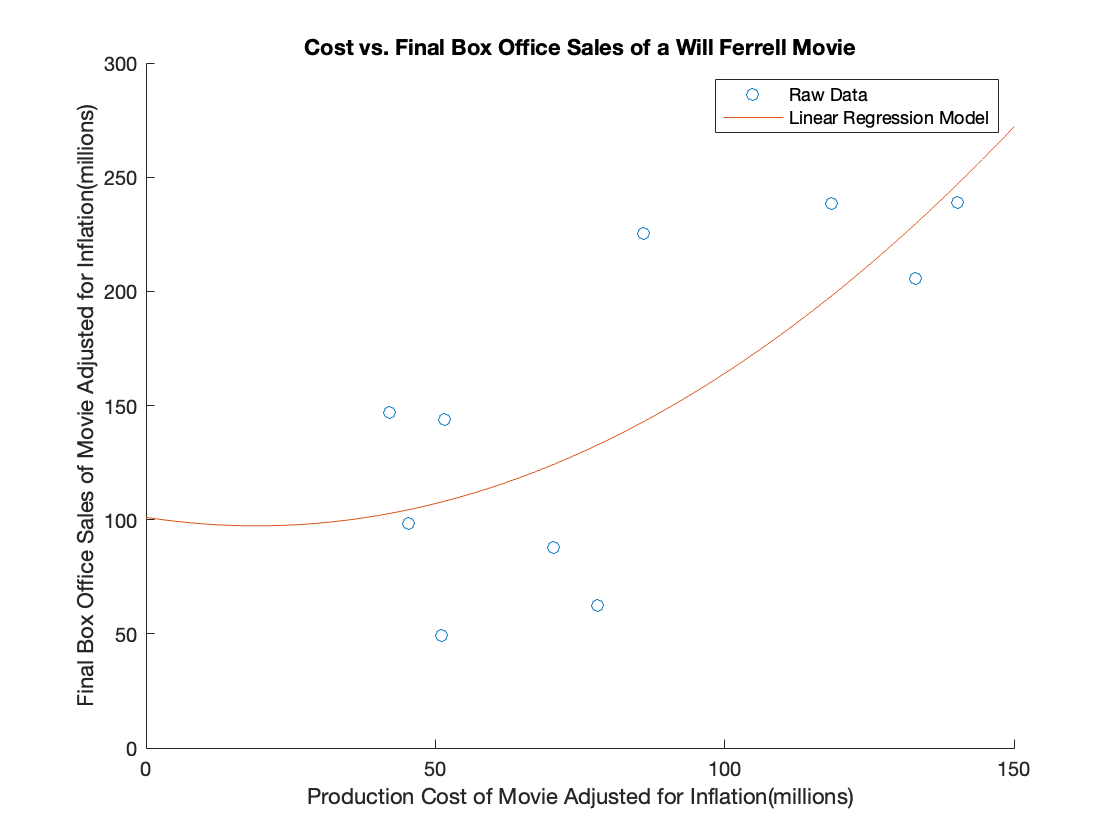
\includegraphics[width=\textwidth]{models/b.png}
\end{figure}
This model seems to fit the data decently well, and if we analyze our least squares error we can see that $E(101.013325, -0.388936, 0.010194) = 22038.897241$.  
This error is clearly slightly less than the error presented for our linear model in \ref{one-variable-linear-model-analysis}, however, there is more to be said.
If we look at the general trend of the model, there appers to be a minimum value that is greater than \$0, which does not make intuitive sense.  If we are thinking about our model in terms of what it means in real life, it clearly does not make sense that a movie with a \$0 budget would have a higher box office revenue than a movie with a budget greater than \$0. 
\\

Other than this issue, our model seems to fit the data well and goes along well with the intuition discussed in \ref{one-variable-linear-model-analysis}, where we said that people may be inclined to believe that the relationship between investment and return is not a linear one.  This model seems to showcase this idea fairly nicely, but it is unclear if it has a non-negligable difference in error from our linear model.  
Because of this and the issue with our minimum box office sales being greater than \$0, we can come to the conclusion that our linear regression model is likely a better fit for this situation than our quadratic one.

\subsection{Two Variable Linear Model}
\subsubsection{Description of Mathematics}
By solving a linear system of two variables, we are trying to build a model of the form
\begin{align*}
    F = a_1 + a_2 T + a_3 B \, ,
\end{align*}
where $F$ is our final box office sales prediction, $T$ is our Rotten Tomatoes score, and $B$ is the production cost of the film. 
\\

In order to find our regression coefficients to minimize the error of our system, we want to solve the system
\begin{align*}
    F_1 &  = a_1 + a_2 T_1 + a_3 B_1 \\  % TODO: formatting here
    F_1 & = a_1 + a_2 T_1 + a_3 B_1 \\
    & \vdots \\
    F_n & = a_1 + a_2 T_n + a_3 B_n \, ,
\end{align*}
where we are solving for the regression coefficients that optimize the model error for $n$ distinct movies.  
Notice we can express this system as a matrix equation of the form
\label{matrix-system-2var-linear}
\begin{align*}
    \begin{bmatrix}
        F_1\\
        F_2 \\
        \vdots \\
        F_n
    \end{bmatrix}
    =
    \begin{bmatrix}
        1 & T_1 & B_1 \\
        1 & T_2 & B_2 \\
        & \vdots & \\
        1 & T_n & B_n
    \end{bmatrix} 
    \begin{bmatrix}
        a_1 \\
        a_2 \\
        a_3
    \end{bmatrix} \, .
\end{align*}
However, notice that we may have that our matrix may not necessarily be solvable.  
Namely, if $n \neq 3$.  
So, we can left multiply both equations by the transpose of $A$, $A^T$, so that we are multiplying by a square matrix. 
This gives us
\begin{align*}
    \begin{bmatrix}
        1 & T_1 & B_1 \\
        1 & T_2 & B_2 \\
        & \vdots & \\
        1 & T_n & B_n
    \end{bmatrix} ^{T}
    \begin{bmatrix}
        F_1\\
        F_2 \\
        \vdots \\
        F_n
    \end{bmatrix}
    =
    \begin{bmatrix}
        1 & T_1 & B_1 \\
        1 & T_2 & B_2 \\
        & \vdots & \\
        1 & T_n & B_n
    \end{bmatrix} ^{T}
    \begin{bmatrix}
        1 & T_1 & B_1 \\
        1 & T_2 & B_2 \\
        & \vdots & \\
        1 & T_n & B_n
    \end{bmatrix}
    \begin{bmatrix}
        a_1 \\
        a_2 \\
        a_3
    \end{bmatrix} \, ,
\end{align*}
which we can see is solvable, since $A^T A$ is a square matrix.  
Hence, if we consider this matrix equation to be of the form $\overrightarrow{b} = A'\overrightarrow{x}$ where $A' = A^T A$, we can solve for $\overrightarrow{x}$ by doing the following:
\begin{align*}
    \overrightarrow{b} = A' \overrightarrow{x} \implies (A')^{-1}\overrightarrow{b} & = (A')^{-1}A' \overrightarrow{x} \\
    & = \mathds{1} \overrightarrow{x} \\
    & = \overrightarrow{x} \, .
\end{align*}

So, we have
\begin{align*}
    \overrightarrow{x} = A^{-1} \overrightarrow{b} \, .
\end{align*}
Hence, if we calculate the value of $(A')^{-1} \overrightarrow{b}$, we will have the values of our coefficients $a_1, a_2, \; \& \; a_3$.

\subsubsection{Applications in Code}
\label{model-code-linear-2-variable}
We are able to solve for our coefficients $a_1, a_2, \; \& \; a_3$ in MATLAB using the methods described in \ref{matrix-system-2var-linear}. 
First, we set up our $A$ matrix and $\overrightarrow{b}$ vector using the following
\begin{lstlisting}
% Set up A matrix and b vector
A = [ones(size(tomato_score)) tomato_score cost];
b = sales;
\end{lstlisting}
Now, we are able to solve for x by using the $\backslash$ operation in MATLAB.  This will automatically left multiply the transpose of A in order to get a solvable matrix.
\begin{lstlisting}
% Solve Ax = b for x
x = A\b;
\end{lstlisting}
Inspecting the results of this operation, we have
\[a_1 = 8.723659, \; a_2 = 0.778640, \; a_3 = 1.306754 \, .\]
Hence, we have our explicit model to be
\[ F = 8.723659 + 0.778640 T + 1.306754 B \, .\]
We can assemble our model in code by doing the following:
\begin{lstlisting}
% Create our model
model = @(t, b) (x(1) + x(2)*t + x(3)*b);
\end{lstlisting}
Now that we have created our model, we can build our visualization similarly to the steps taken in \ref{model-plotting} with the only difference is that instead of creating a "continuous" set of points, we have to build a 2-D mesh that acts this same way.  
We can do this using the \texttt{meshgrid} function in MATLAB.
\begin{lstlisting}
% Build our model visualization
[X, Y] = meshgrid(0:1:100, 0:1:200);
model_visualization = model(X, Y);
\end{lstlisting}
Similarly to what we did to plot in \ref{model-plotting}, we can plot our visualization of the model.  
We can use the \texttt{scatter} \texttt{surf} functions in MATLAB to show the model and our raw data as follows:
\begin{lstlisting}
scatter3(tomato_score, cost, sales, 'filled', 'DisplayName', 'Raw Data');
surf(X, Y, model_visualization, 'DisplayName', 'Regression Model');
\end{lstlisting}

\newpage
\subsubsection{Model Analysis}
We obtain the following model from the code in \ref{model-code-linear-2-variable}.
\label{two-variable-linear-plot}
\begin{figure}[H]
    \centering 
    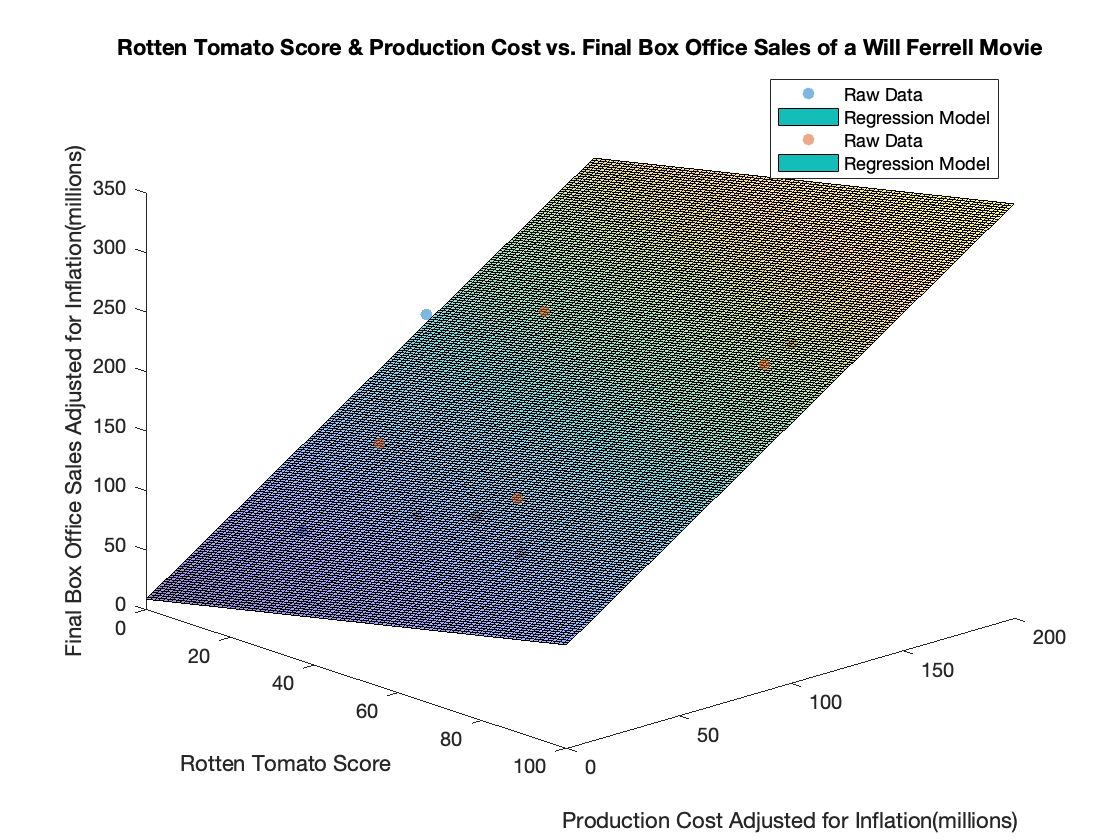
\includegraphics[width=\textwidth]{models/c-2.png}
\end{figure}
Looking at the visualization of our model, it appears to be a good fit for the presented data.  
The model also seems to make intuitive sense.  
We can see as the Rotten Tomatoes score increases, so does the anticipated final box office sales.  
Similarly, as the production cost increases, so does the final box office sales.
We can also see from the model that the production cost seems to effect the projected final box office sales in a way that is stronger than the Rotten Tomatoes score.  
This is an interesting observation, as it seems to indicate that production cost is a more important factor in determing box office success than reviews. 
However, this may not be as good for predicting the results of an upcoming movie since there will not be a Rotten Tomatoes score for such a movie, whereas the production cost may be available. 
\\

We can evaluate the least squares error of our model to see that $E(8.723659,0.778640,1.306754) = 19123.077237$.  Given the scale of numbers we are working with, this seems to be a fairly reasonable error.  Given that our model makes clear intuitive sense and has a reasonably low least squares error, we can come to the conclusion that this model is good for predicting the final box office sales given the production cost and Rotten Tomatoes score of a Will Ferrell movie.

\subsection{Two Variable Quadratic Model}
\subsubsection{Description of Mathematics}
\label{matrix-system-2var-quadratic}
In creating a two variable quadratic model, we would like to build a model of the form
\begin{align*}
    F = a_1 + a_2 T + a_3 B + a_4 T^2 + a_5 B^2 + a_6 TB \, ,
\end{align*}
where F is our final box office sales prediction, T is our Rotten Tomatoes score, and B is the production cost of the film.
We can extend the ideas discussed in \ref{matrix-system-2var-linear} to set up a matrix equation that we can use to solve for our regression coefficients $a_1, a_2, a_3, a_4, a_5, \; \& \; a_6$.  
Thus, we have
\begin{align*}
    \begin{bmatrix}
        F_1\\
        F_2 \\
        \vdots \\
        F_n
    \end{bmatrix}
    =
    \begin{bmatrix}
        1 & T_1 & B_1 & T_1^2 & B_1^2 & T_1 B_1\\
        1 & T_2 & B_2 & T_1^2 & B_2^2 & T_2 B_2\\
        & & & \vdots & \\
        1 & T_n & B_n & T_n^2 & B_n^2 & T_n B_n
    \end{bmatrix} 
    \begin{bmatrix}
        a_1 \\
        a_2 \\
        a_3 \\
        a_4 \\
        a_5 \\
        a_6
    \end{bmatrix} \, .
\end{align*}
Similarly as discussed previously, if $n \neq 6$, then we see that we can solve the matrix by left multiplying the LHS and RHS by the transpose of our $A$ matrix.  
Thus, we have a way to find our regression coefficients $a_1, a_2, a_3, a_4, a_5, \; \& \; a_6$.


\subsubsection{Applications in Code}
\label{model-code-quadratic-2-variable}
Similarly to what was discussed in \ref{model-code-linear-2-variable}, we can extend our $A$ matrix in MATLAB to be representative of what we have in \ref{matrix-system-2var-quadratic}.  
Thus, in code we have the following:
\begin{lstlisting}
% Set up A matrix
A = [ones(size(tomato_score)) tomato_score cost (tomato_score.^2) (cost.^2) (tomato_score.*cost)];
\end{lstlisting}
Solving $A^T A \overrightarrow{x} = A^T \overrightarrow{b}$ using the $\backslash$ operator, we can see that we have
\[a_1 = -27.495717, a_2 = 0.386540, a_3 = 2.179780, a_4 = 0.016820, a_5 = -0.001396, a_6 = -0.013145 \, .\]
Hence, we have our explicit model to be 
\[ F = -27.495717 + 0.386540 T + 2.179780 B + 0.016820 T^2 + -0.001396 B^2 + -0.013145 TB \, .\]
Thus, we can build our model similarly to what we had done for the 2 variable linear model.
\begin{lstlisting}
% Build our model
model = @(t, b)(x(1) + x(2)*t + x(3)*b + x(4)*(t.^2) + x(5)*(b.^2) + x(6)*(t.*b));
\end{lstlisting}
We are then able to build and plot our visualization the same way we had done in \ref{model-code-linear-2-variable}.

\newpage
\subsubsection{Model Analysis}
We obtain the following model from \ref{model-code-quadratic-2-variable}.
\label{two-variable-quadratic-plot}
\begin{figure}[H]
    \centering 
    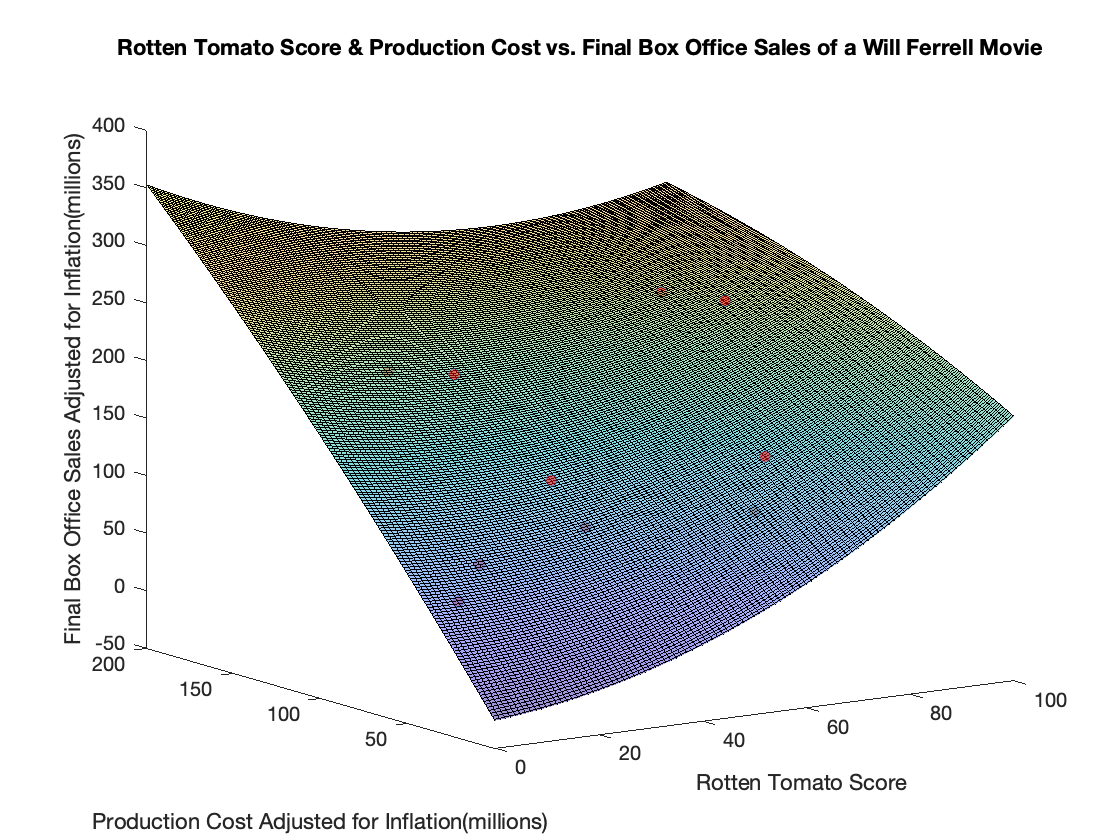
\includegraphics[width=\textwidth]{models/d.png}
\end{figure}
We can see that this model seems to fit the data fairly well, however it does not necessarily make intuitive sense upon further inspection. 
For example, if we fix a production cost of $\$ 200$ million, we see that our model predicts a higher box office sales at a Rotten Tomatoes score of $0$ than a Rotten Tomatoes score of $20$.
If we evaluate the least squares error of our model, we can see that we have an error of $18409.715164$.  
Despite this error being fairly low given the context of our dataset, the fact that this model does not make intuitive sense means that it is likely not the greatest representation of the overall relationship between Rotten Tomatoes score, Production Cost, and Final Box Office sales of a Will Ferrell movie.

\subsection{Three Variable Linear Model}
\subsubsection{Description of Mathematics}
In building a 3 variable linear model, we want to build an equation of the form
\label{three-var-linear-equation}
\begin{align*}
    F = a_1 + a_2 T + a_3 W + a_4 B \, ,
\end{align*}
where $F$ is our final box office sales prediction, $W$ is the age of Will Ferrell at the time of release, $T$ is our Rotten Tomatoes score, and $B$ is the production cost of the film. 
\\

The process for solving for our regression coefficients is quite similar to what was presented in \ref{matrix-system-2var-linear}.  
We can extend these ideas to build a matrix equation of the form $A \overrightarrow{x} = \overrightarrow{b}$.  Hence, we have our matrix equation to be
\label{matrix-system-3var-linear}
\begin{align*}
    \begin{bmatrix}
        F_1\\
        F_2 \\
        \vdots \\
        F_n
    \end{bmatrix}
    =
    \begin{bmatrix}
        1 & T_1 & W_1 & B_1 \\
        1 & T_2 & W_2 & B_2 \\
        & & \vdots & \\
        1 & T_n & W_n & B_n
    \end{bmatrix} 
    \begin{bmatrix}
        a_1 \\
        a_2 \\
        a_3 \\
        a_4
    \end{bmatrix} \, .
\end{align*}
Which we can solve for our optimal coefficients by left multiplying the transpose of our $A$ matrix as discussed previously.  
Hence, we have a way to solve for our regression coefficients.
\subsubsection{Applications in Code}
The code used to build our model is very similar to what we had presented in \ref{model-code-linear-2-variable}, with the exception of two minor changes.  The first change is expanding our $A$ matrix to account for our new variable.
\begin{lstlisting}
% Set up A matrix
A = [ones(size(tomato_score)) tomato_score age cost];
\end{lstlisting}
The second change is when we actually build our model.  We need our equation to reflect that presented in \ref{three-var-linear-equation}.  
Solving our matrix equation for $\overrightarrow{x}$, we have
\[ a_1 = -109.707546, a_2 = 0.953030, a_3 = 2.771033, a_4 = 1.196892 \, .\]
Thus, we have our explicit model to be
\[ F = -109.707546 + 0.953030 T + 2.771033 W + 1.196892 B \, .\]
The representation of this model in code is as follows:
\begin{lstlisting}
model = @(t, a, b)(x(1) + x(2)*t + x(3)*a + x(4)*b);
\end{lstlisting}
\textbf{Note:} We are unable to plot such a model, since it is a model of 3 dimensions and we cannot plot a 4th dimension representing the output.

\subsubsection{Model Analysis} 
Despite not having a visual representation of our model, we can still draw some interesting conclusions regarding it.  
This model has a relatively high least squares error of $565319.514600$.  
This may be due to the introduction of age.  
Intuitively, it does not make sense for the relationship between Will Ferrell's age and the final box office sales of his movies to be related in a linear fashion.  
If any intuitive conclusion was to be made, it would likely be that his box office sales would be related in a more quadratic fashion to his age.  
This is because you may expect an actor to "peak" at a certain age, where they end up producing the most commercially successful movies.
Though it is worth noting that this is most definitely a massive oversimplification of this relationship.
Due to the clear unintuitive nature and high error of this model, it is likely not a great one to predict the success of a Will Ferrell movie.



\section{\centering Summary and Conclusions}
Following our discussion and analysis of the 5 presented models, we can conclude that the best model is likely the two variable linear model.  
This model, despite not having the lowest error, made the most intuitive sense among the models presented.
As discussed in our analysis, the model depended strongly on the production cost of said movie. 
While the Rotten Tomatoes score did not play as important of a role as production cost, it had an important effect on our overall model and the regression coefficients for these followed general intuition.
\\

We can use our model to predict the success of the movie \textit{Strays}(2023).  Knowing that \textit{Strays} had a budget of \$46 million dollars and with a Rotten Tomatoes score of 54\%, we can plug these values into the model,
\[ F = 8.723659 +  0.778640T + 1.306754 B \, ,\]
to see a predicted final box office result of \$110.88 million USD.
\end{document}